\documentclass[a4paper,10pt]{report}
\usepackage{graphicx}
\usepackage[polish]{babel}
\usepackage[utf8]{inputenc}
\usepackage{polski}
\usepackage[T1]{fontenc}
\usepackage{indentfirst}
\usepackage{amsmath}
\usepackage{verbatim}
\usepackage{booktabs}
\usepackage{color}
\usepackage[usenames,dvipsnames,svgnames]{xcolor}
\usepackage{geometry}
\geometry{verbose,lmargin=3cm,rmargin=3cm}
\usepackage{utopia}
\frenchspacing

%opening
\title{Rozpoznawanie relacji sematycznych w tekscie, porzez klasyfikację kontekstu relacji przy pomocy klasyfikatora \textbf{CRF}}
\author{Jakub A. Gramsz \\ Michał Krautforst}
\date{24 stycznia 2014}

\begin{document}
\renewcommand{\figurename}{Wykres}
\renewcommand{\chaptername}{}

\maketitle
\tableofcontents

\chapter{Wstęp} % to wszystko jes oczywiście do przeredagowania, nic nie jest jeszcze ostateczną wersją.

\section{Klasyfikator CRF} 

\subsection{Motywacja}

Klasyfikator utworzony pod kątem segmentacji i znakowania danych sekwencyjnych.

Często wykorzystywane w przetwarzaniu języka naturalnego.

Stosunkowo młoda metoda klasyfikacji, wykazująca potencjał do badań.

Wysoka jakość klasyfikacji otrzymana przy oznaczaniu nazw własnych w tekstach.

\subsection{Charakterystyka klasyfikatora}

Klasyfikator CRF został zaporoponowany aby przetwaorzać sekwencje w obu kierunkach \cite{lafferty2001crf}.

\section{Rozpoznanie literatury}



\chapter{Praca badawcza}

\section{Implementacja}

\noindent Poniżej przedstawiamy zadania.
\begin{enumerate}
 \item Wydobycie par hiponim-hiperonim o zadanej odległości między sobą wprost z bazy Słowosieci. % skryp to wyciągania par hiponim-hiperonim dla zadanej odległości
 \item Budowa grafu relacji hiperonimi. % graf relacji hiperonimi (działa za wolno)
 \item Oznaczenie otrzymanych par w zadanym korupusie. % skrypt oznaczający wyciągnięte pary w zadanym korpusie
 \item Podział korpusu na zbiór uczący oraz testujący. % skrypt dzielacy oznaczony korpus na dane uczace i testujace
 \item Wydobycie oznaczonych kontekstow. % skrypt co wyciagania oznaczonych kontekstow
 \item Wypisywanie przykładów false positive skrypt wypisujacy przyklady false positive.
 \item Dobór cech dla klasyfikatora \textbf{CRF}.  % badanie wpływu doboru cech
 
 \item Wyznacznanie odległości pomiędzy parami oznaczonymi poprzez klasyfikator (pośrednio oznaczonymi poprzez kontekst).  % skyrp do sprawdzania odległości wyodrębionych par
\end{enumerate}

\section{Badania}

\subsection{Zbiór uczący}

Zbiór uczący stanowią zdania pochodzące z korpusów języka polskiego z oznaczonymi kontekstami par słów znajdujących się w relacji hiperonimi znajdujących się w różnych odległościach od siebie (1 do 3) w słowosieci. Każdy token opisany wektorem cech.

\begin{itemize}
 \item walidację krzyżową dla 2, 3 i 10 foldów.
 \item dla długości kontekstów 5, 10, 15
 \item dla par hiponim-hiperonim o odległościach 1, 2, 3.
\end{itemize}

\chapter{Wyniki i wnioski}

\section{Wyniki}

\begin{figure}[h]
\centering
 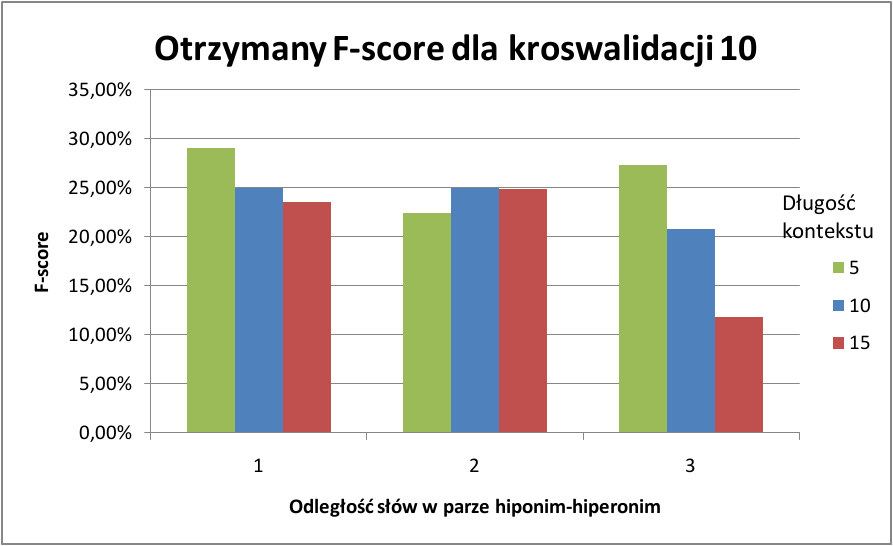
\includegraphics[width=13cm]{img/image003.png}
 \caption{}
\label{fig:wykres}
\end{figure} 

\section{Wnioski}

Skorzystanie z par hiponim-hiperonim o większej odległości powoduje spadek precyzji bez zmian kompletności

Długość kontekstu wpływa na liczbę wygenerowanych przypadków pozytywnych (najlepszy wynik dla 10, dłuższe konteksty nie polepszają już wyników)

Manipulacja cechami niezauważalnie wpływa na wyniki (cech powinno być możliwie dużo)

Zmniejszenie liczby negatywnych przypadków pogarsza jakość klasyfikacji. Należałoby zrównoważyć proporcje liczby przypadków pozytywnych i negatywnych, jednak trudne jest określenie kryterium.


Klasyfikacja cechuje się wysoką precyzją, mimo zróżnicowanych przypadków pozytywnych oraz rzadkiej powtarzalności kontekstów

Zaproponowana metoda odnajdowania relacji sematycznych w tekście poprzez oznaczanie ich kontekstów, nie przynosi zadowalających rezultatów, niemniej jednak może stanowić dobry wstęp na podstawie, którego innymi metodami można by proces ten kontynuować. Przykładowo oznaczone konteksty można by grupować na podstawie ich podobieństwa a następnie wyciągać z nich bardziej ogólne wzorce.

%Bibliografia
\bibliographystyle{abbrv}
\nocite{*}
\bibliography{sem-rel-crf}

\end{document}
